\documentclass[english]{beamer}
\usepackage[english]{babel}
\usepackage[utf8]{inputenx}
\usepackage[T1]{fontenc}      % Font encoding
\usepackage{lmodern}          % lmodern font, correctly copyable characters in pdf

\usetheme[
  bullet=circle,                  % Use circles instead of squares for bullets
  titleline=false,                % Show a line below the frame
  alternativetitlepage=true,      % Use the fancy title
  titlepagelogo=logo-sapienza,    % Logo for the first slide
  watermark=watermark-diag,   % Watermark used in every slide
  watermarkheight=20px,           % Desired height of the watermark
  watermarkheightmult=6,          % Watermark image is actually x times bigger
  displayauthoronfooter=true,     % Display author name in the footer
]{Roma}
\watermarkoff
\author{Dario Loi, Davide Marincione, Benjamin Barda}
\title{Mine-RPN}
\subtitle{Or how we were able to recognize pigs et. familia in Minecraft}
\institute{Bachelor's degree in\\Applied Computer Science and Artificial Intelligence\\Sapienza, University of Rome}
\date{A. Y. 2021 - 2022}

\begin{document}

\begin{frame}[t,plain]
\titlepage
\end{frame}

\section{Who?}
\begin{frame}{Breaking the ice}
  FACCIAMO QUALCOSA DI SCEMO
\end{frame}
\section{What, why?}
\begin{frame}{Faster RCNN}
	\begin{columns}
	    
	    \begin{column}{0.5\textwidth}
	      Developed in 2015 by Facebook's researches, Faster-RCNN is still today an industry standard thanks to it's accuracy and performance, getting a step closer to real time object detection
	    \end{column}
	
	    \begin{column}{0.5\textwidth}
	      \begin{figure}
	        \centering
	            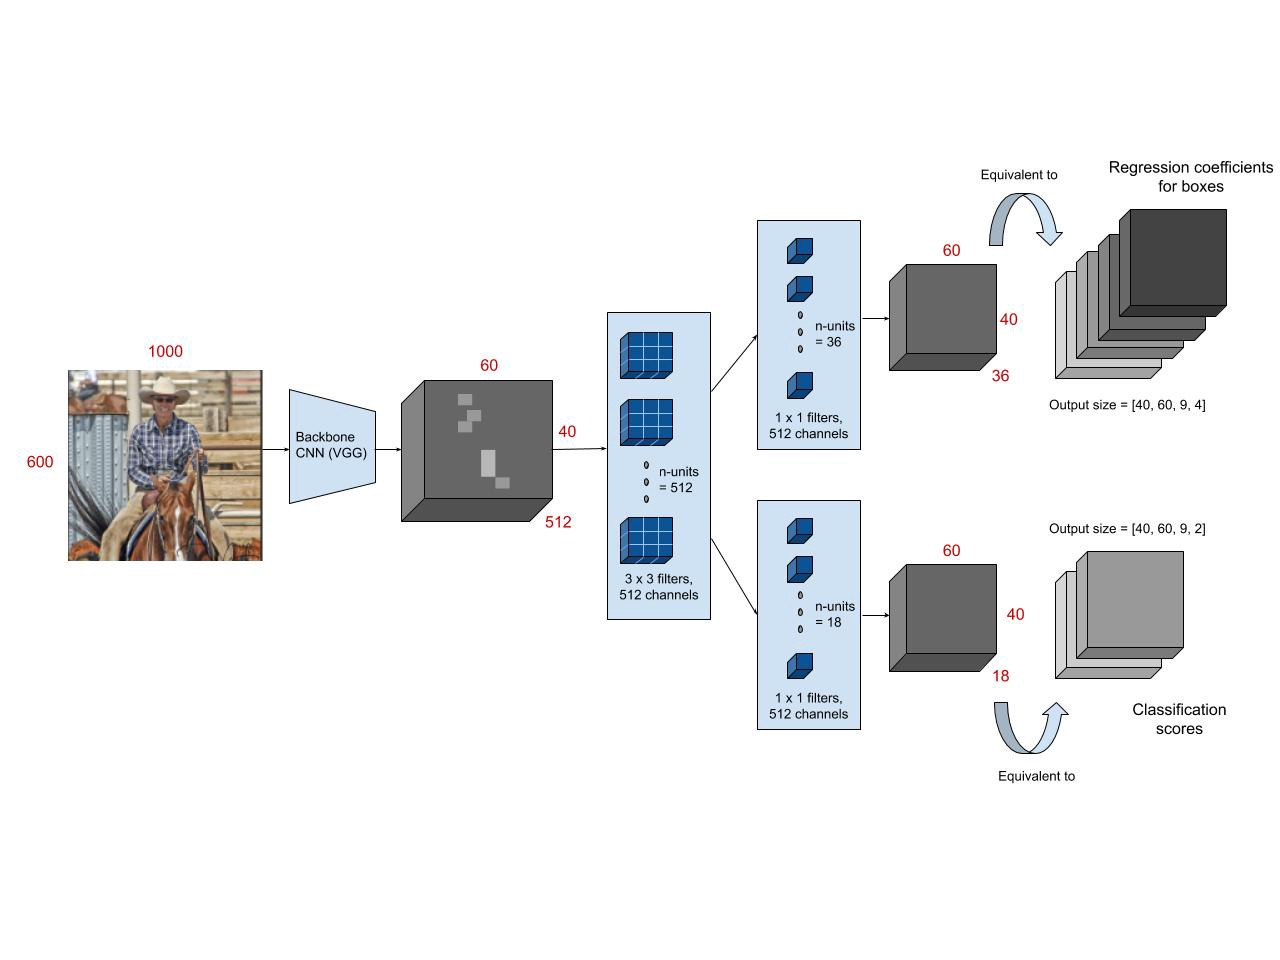
\includegraphics[width=1.0\textwidth]{../images/rpn_schema.jpeg}
	            \caption{Faster-RCNN architechture.}
	        \end{figure}
	    \end{column}
	  \end{columns}
\end{frame}

\begin{frame}{Why minecraft?}

  \begin{columns}
    
    \begin{column}{0.5\textwidth}
      Minecraft has several desirable qualities:
      \begin{itemize}
        \item Simple graphics.
        \item Sandbox.
        \item Available to every team member.
        \item Distinguishable entity silhouettes.
      \end{itemize}
    \end{column}

    \begin{column}{0.5\textwidth}
      \begin{figure}
        \centering
            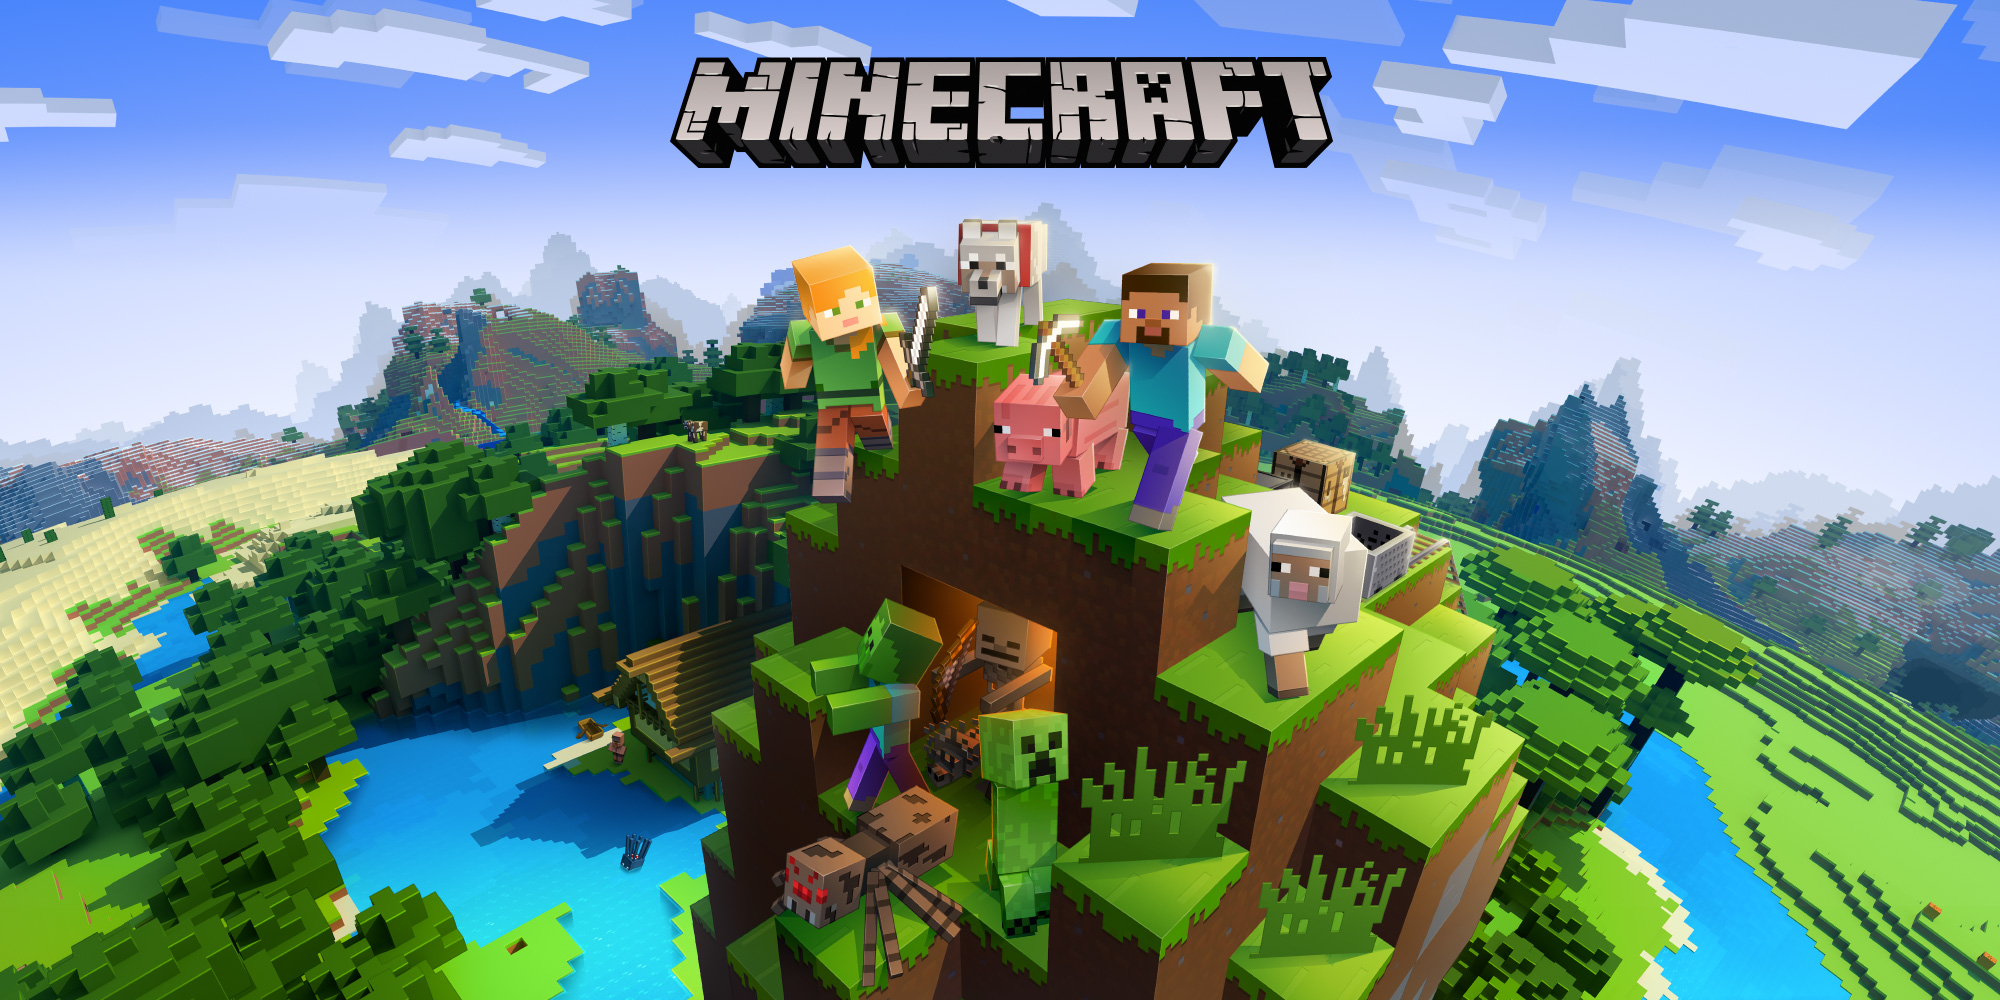
\includegraphics[width=1.0\textwidth]{images/minecraft.jpg}
            \caption{A Minecraft promotional image.}
        \end{figure}
    \end{column}

  \end{columns}

\end{frame}

\section{Dataset}
\begin{frame}{Behold, data!}
  \begin{figure}[h]
      \centering
      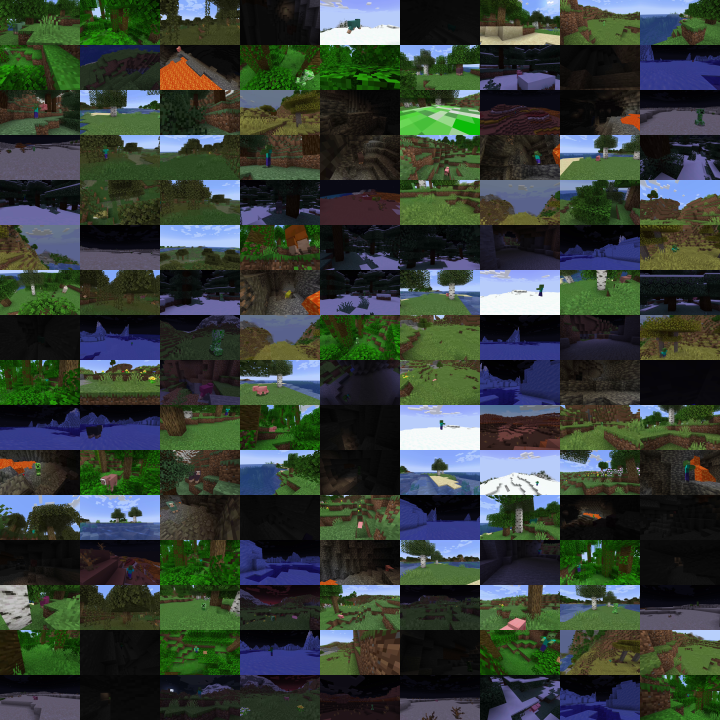
\includegraphics[width=0.5\textwidth]{../images/dtset_repr.png}
      \caption{A representative chunk of our dataset}
  \end{figure}
\end{frame}

\begin{frame}{Tool}
  \begin{columns}
    \begin{column}{0.5\textwidth}
      How to label 4000 images?
      \begin{enumerate}
        \item Load image
        \item Create box / purge
        \item Next
      \end{enumerate}
    \end{column}

    \begin{column}{0.5\textwidth}
      \begin{figure}[h]
        \centering
        \vspace*{-1cm}
        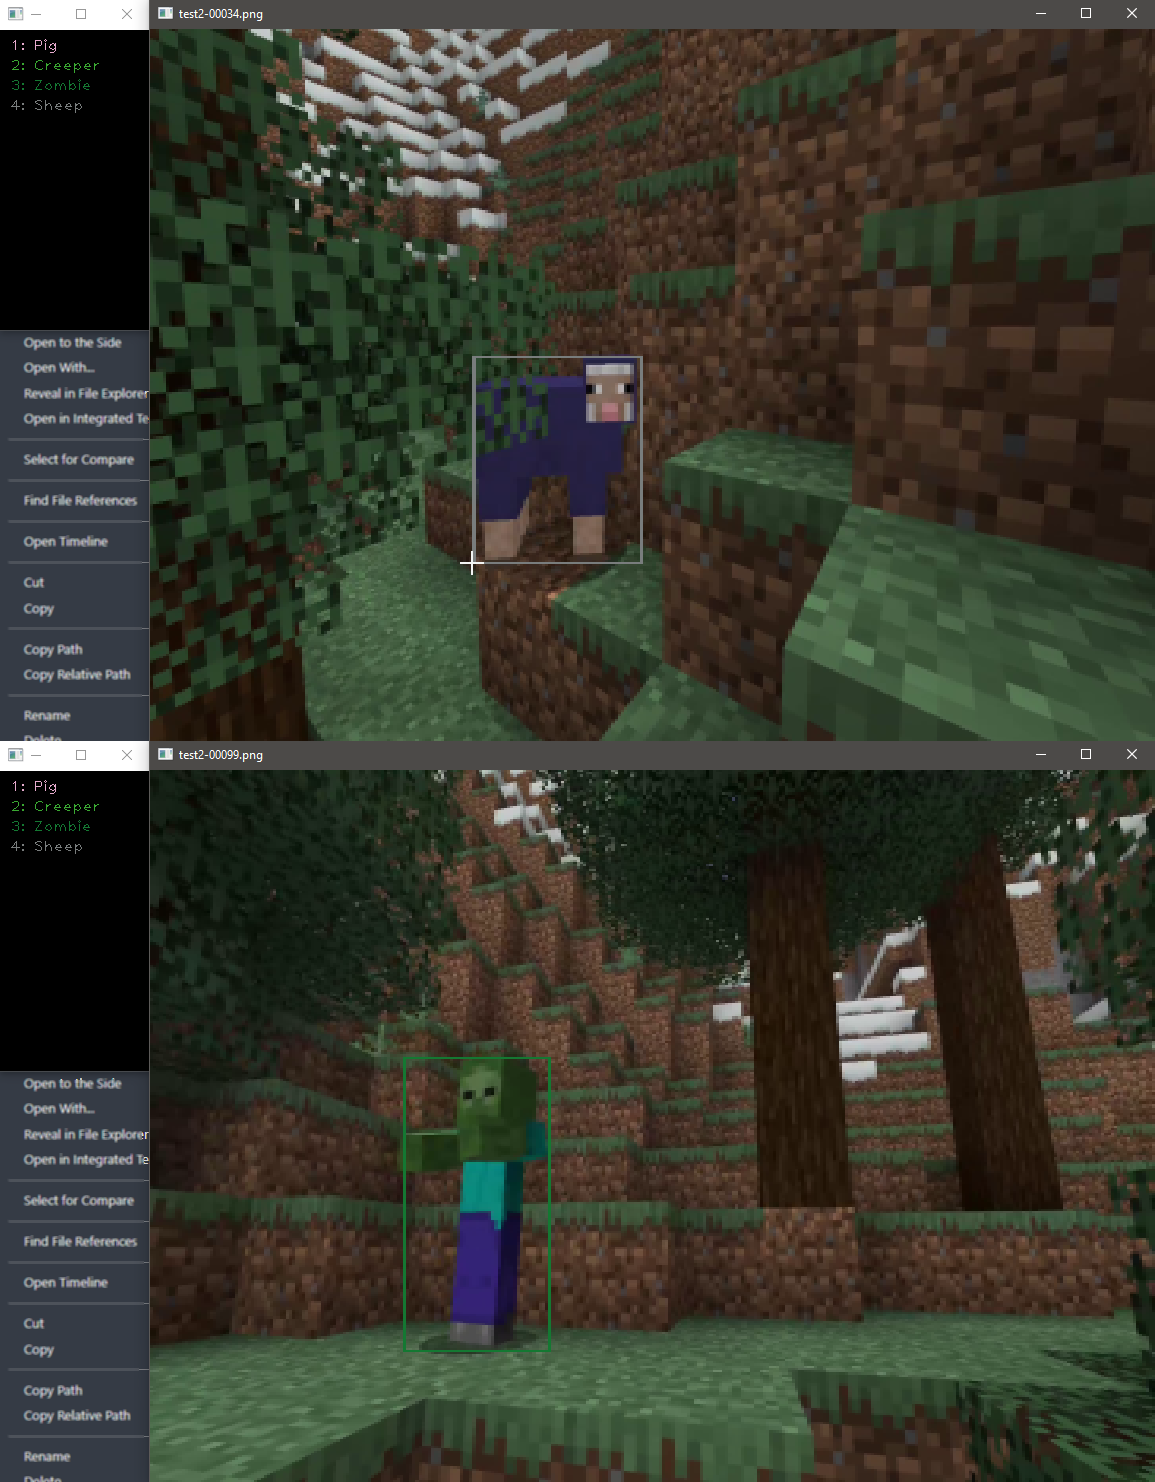
\includegraphics[width=0.9\textwidth]{../images/dataset_tool_show.png}
        \caption{BBoxing in our tool}
      \end{figure}
    \end{column}
  \end{columns}
\end{frame}

\section{Architectures}
\begin{frame}{Our Backbone}
  \begin{columns}
    
    \begin{column}{0.5\textwidth}
      The backbone is the convolutional \emph{heart} of our model, it is:
      \begin{itemize}
        \item Blazingly fast.
        \item Adaptable to any resolution.
      \end{itemize}
      While also offering:
      \begin{itemize}
        \item A 92\% accuracy when used as a Classifier.
        \item A mean training time of $\approx2h$.
      \end{itemize}
    \end{column}

    \begin{column}{0.5\textwidth}
      \begin{figure}
        \centering
            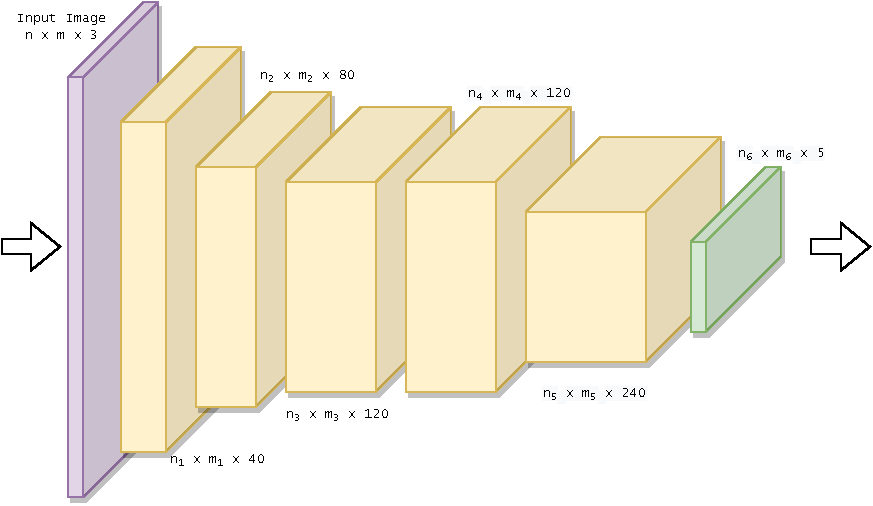
\includegraphics[width=1.0\textwidth]{images/backbone.pdf}
            \caption{Our backbone.}
        \end{figure}
    \end{column}

  \end{columns}
\end{frame}

\begin{frame}{Our RPN}
  \begin{columns}
    
    \begin{column}{0.5\textwidth}
      Our RPN network extends our Backbone and is composed mainly of two twin layers:
      \begin{enumerate}
        \item A Classification layer.
        \item A Regression layer.
      \end{enumerate}
      Before feeding data into those, it also performs some pre-processing:
      \begin{itemize}
        \item Anchor Splashing.
        \item Base convolution.
        \item Flattening (how do we get to fully connected otherwise?)
      \end{itemize}
    \end{column}

    \begin{column}{0.5\textwidth}
      \begin{figure}
        \centering
            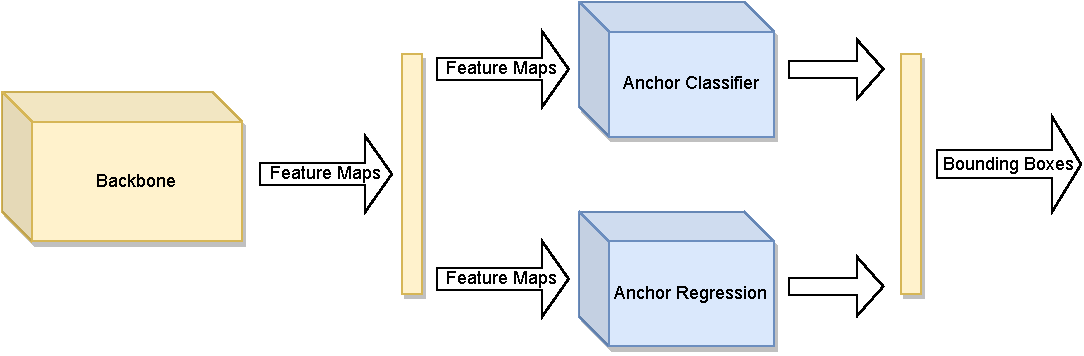
\includegraphics[width=1.0\textwidth]{images/network.pdf}
            \caption{Our network's proposal layer.}
        \end{figure}
    \end{column}

  \end{columns}
\end{frame}

\section{Conclusions}
\begin{frame}{Behold, data!}
  \begin{figure}[h]
      \centering
      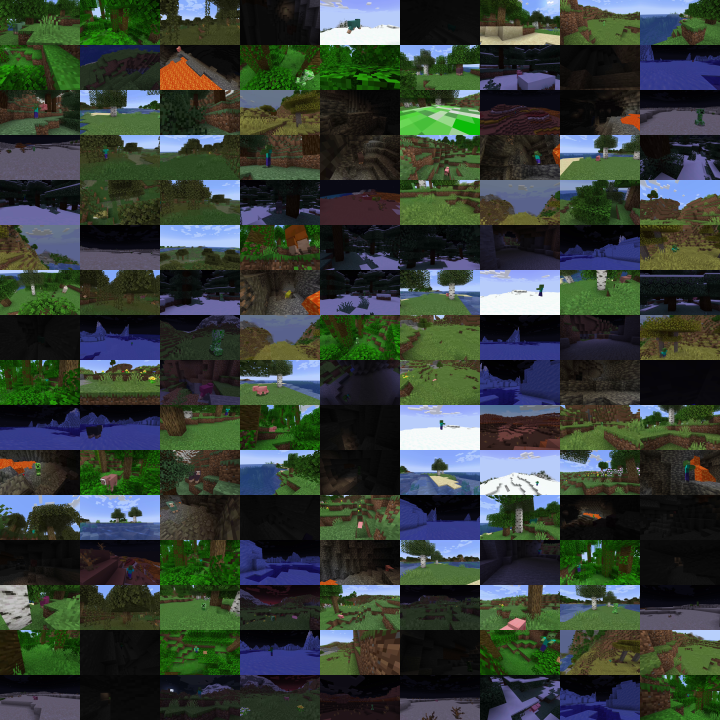
\includegraphics[width=0.5\textwidth]{../images/dtset_repr.png}
      \caption{A representative chunk of our dataset}
  \end{figure}
\end{frame}



\end{document}